\documentclass{article}
\usepackage{fullpage}
\usepackage{times}
\usepackage{fancyhdr,graphicx,amsmath,amssymb}
\usepackage[ruled,vlined]{algorithm2e}
\include{pythonlisting}

\usepackage{multirow}
\usepackage{graphicx}
\usepackage{blindtext}

\usepackage{subcaption}

\usepackage{arxiv}
\usepackage{listings}
\lstset
{ %Formatting for code in appendix
    language=C,
    basicstyle=\footnotesize,
    numbers=left,
    firstnumber= 0,
    stepnumber=1,
    showstringspaces=false,
    tabsize=1,
    breaklines=true,
    breakatwhitespace=false,
    xleftmargin=0.04\textwidth,
}
\usepackage[utf8]{inputenc} % allow utf-8 input
\usepackage[T1]{fontenc}    % use 8-bit T1 fonts
\usepackage{hyperref}       % hyperlinks
\usepackage{url}            % simple URL typesetting
\usepackage{booktabs}       % professional-quality tables
\usepackage{amsfonts}       % blackboard math symbols
\usepackage{nicefrac}       % compact symbols for 1/2, etc.
\usepackage{microtype}      % microtypography
\usepackage{lipsum}
\newcommand*\samethanks[1][\value{footnote}]{\footnotemark[#1]}
\newcommand{\tabincell}[2]{\begin{tabular}{@{}#1@{}}#2\end{tabular}}
\title{Systematic Predicate Abstraction using Deep Learning}


\author{
  Name \thanks{All contributions are considered equal.}\\
  Department of \\
   University\\
  Address \\
  \texttt{xxx@xxx} \\
  %% examples of more authors
   \And
 Name \samethanks\\
  Department of \\
   University\\
  Address \\
  \texttt{xxx@xxx} \\
     \And
 Name \samethanks\\
  Department of \\
   University\\
  Address \\
  \texttt{xxx@xxx} \\
  %% \AND
  %% Coauthor \\
  %% Affiliation \\
  %% Address \\
  %% \texttt{email} \\
  %% \And
  %% Coauthor \\
  %% Affiliation \\
  %% Address \\
  %% \texttt{email} \\
  %% \And
  %% Coauthor \\
  %% Affiliation \\
  %% Address \\
  %% \texttt{email} \\
}

\begin{document}
\maketitle

\begin{abstract}
Systematic Predicate Abstraction using Deep Learning
\end{abstract}


% keywords can be removed
\keywords{First keyword \and Second keyword \and More}


\section{Introduction}
Systematic Predicate Abstraction using Deep Learning

Reduce CEGAR iterations.

Summarize the pipline:

\section{Background}
---
\subsection{Abstraction Based Model Checking}
---
\subsection{CEGAR}
---
\subsection{Abstract Interpolation}
---
\section{Problem Overview}
---

\section{Program representation}
Eldarica can take SMT and C format programs as inputs and transform the programs to intermediate horn clause format [cite]. In this format, the semantics are transformed to horn clauses. By using horn clauses as inputs, our method can adapt to many verification problems because many verification problems can be transformed to SMT format and eventually to horn clauses. We have an example in Figure \ref{while-C-program} and \ref{while-C-horn-clauses} to explain how the horn clauses capture the semantics of the program.

In Figure \ref{while-C-program}, we have a simple while loop C program which assumes variable $x$ and $y$ equal to external input Integer $n$ and $n\geq 0$. The assertion is $y==0$. The corresponding Horn clauses can be found in  Figure \ref{while-C-horn-clauses}. Every line is consists of $Head:-Body,[constraint]$. For example, in line 0, $Head$ is $inv\_main4(x, y)$ which means in control location $while(x!=0)$ in the main function and there are two variables $x$ and $y$ inside. $Body$ is empty here because this is the initial state of the program. The $constraint$ is $n \geq 0 \wedge x = n \wedge n = 0 \wedge y = n$ which comes from the $assume(x==n\&\&y==n\&\&n>=0)$ in the C program. Line 0 means in control location $while(x!=0)$, there are two variables $x$, and $y$, which satisfy the $constraint$. In line 1, The body is not empty, this means that there is a transition from body to head and this transition satisfy the $constraint$. Line 1 means from control location $while(x!=0)$ to next iteration, it must satisfy that, $x!=0$ and in the new iteration, the variables $arg1$ and $arg2$ in the control location $while(x!=0)$ must equal to $x-1$ and $y-1$, (values of $x,y$ come from last iteration). Line 2 transforms the semantic of assertion $y==0$ to horn clauses. Line 2 means that from control  location $while(x!=0)$ to false state, in the control location $while(x!=0)$ , the variable $x$ is 0 and $y$ satisfy $y!=0$.


\begin{figure}[h]
\begin{subfigure}[b]{0.4\textwidth}
\begin{lstlisting}
extern int n;
void main(){
    int x,y;
    assume(x==n&&y==n&&n>=0);
    while(x!=0){
        x--;
        y--;
    }
    assert(y==0);
}
\end{lstlisting}\subcaption{An input example: C program}\label{while-C-program}
\end{subfigure}
\begin{subfigure}[b]{0.6\textwidth}
\begin{lstlisting}
inv_main4(x, y) :- ,[n >= 0 & x = n & 0 = n & y = n].
inv_main4(arg1, arg2) :- inv_main4(x, y), [x != 0 & x + -1 = arg1 & y + -1 = arg2 & n = 0].
false :- inv_main4(0, y), [y != 0].
\end{lstlisting}\subcaption{Horn clauses for C program}\label{while-C-horn-clauses}
  \end{subfigure}
  \caption{}
\end{figure}

How to transform program semantics to horn clauses and why it can be transformed in this way can be found in [cite]. Our main purpose is to use this horn clauses format as input of deep learning structure to select predicates to build valid abstract transition systems for model checkers. 

Text streamed Horn clauses as inputs are not enough to make neural networks to understand the semantics because text-level embedding cannot capture the structural information included in the horn clauses. Therefore, we represent horn clauses by a graph which contains both control flow and data flow information, then we embed the graph to represent the original program.

The graph to represent horn clauses in Figure \ref{while-C-horn-clauses} is in Figure .


Formally, the graph consists of five categories of nodes, two categories of hyperedges, and six categories of edges. The graph is defined as $G=(V_{CL},V_{Arg},V_{C},V_{Op},V_{FV},HE_{CF},HE_{DF},E_{CFI},E_{CFO},E_{DFI},E_{DFO},E_{CD},E_{Arg})$, in which $V_{CL}=\{cl_{Initial},cl_{Main_{k}},cl_{false}\}$ is control location node set, $V_{Arg}=\{Arg_{k}\}$ is argument set, $V_{C}$ is constant value set, $V_{Op}=\{+,-,==,...\}$ is operator set,$V_{FV}=\{v_{k}\}$ is free variables set. $k$ is a positive integer. $HE_{CF}$ is a set of Guarded control flow hyper edges. it is used between two control locations. it takes two inputs, a control location $cl_{Initial}$ or $cl_{Mian_{k}}$ and a boolean value from operator. It has a control flow out edge $e_{CFO}$ (one element from $E_{CFO}$) connected to next control location node. Similarly, $HE_{DF}$ is a set of Guarded data flow hyper edges. It guards the data flow from $Body$ to $Head$. It takes two inputs, a value from argument $Arg_{k}$ or free variable $v_{k}$ and a boolean value and has a data flow out edge $e_{DFO}$ (one element from $E_{DFO}$) connected to next operator or argument node. $E_{CFI},E_{CFO}$ are control flow in and control flow out edges, they are only used when there are connections between nodes and guarded control flow hyperedges. similarly, $E_{DFI},E_{DFO}$ are data flow in and out edges, they are only corresponding to guarded data flow hyperedges. $E_{CD}$ is condition edge. It connects boolean operator to the hyperedges to send boolean values to the hyperedges. $E_{Arg}$ is argument edge. It connects arguments to corresponding control location node. We use lower case to represent one elements in the set. For example $v_{CL}$ means one control location node from $V_{CL}$.


The summary of $G$'s elements is shown in Table \ref{GraphDescription}
\begin{table}\caption{Graph elements description} \label{GraphDescription}
\begin{center}
\begin{tabular}{lllll}
\hline
Graph elements & Name & Elements & Inputs & Outputs \\
\hline
$V_{CL}$  & Control location node            & $CL_{Initial},CL_{Main_{k}},CL_{false}$ & $v_{CL}$ & $he_{CF}$\\
$V_{Arg}$ & Argument node                    & $Arg_{k}$                               &  $v_{OP}$, $v_{Arg}$, $v_{FV}$, or $v_{C}$ &\\
$V_{C}$   & Constant node                    & Constants                               & - &\\
$V_{Op}$  & Operator node                    & Arithmetic and boolean operators        & - &\\
$V_{FV}$  & Free Variable node               & Free variables                          & -  & variable\\
$HE_{CF}$ & Guarded control flow hyperedge   & -                                       & $v_{OP}$ or $v_{C}$,$v_{CL}$ & $v_{CL}$\\
$HE_{DF}$ & Guarded data flow hyperedge      & -                                       & $v_{OP}$ or $v_{C}$,$v_{Arg}$ or $v_{FV}$ & $v_{Arg}$\\
$E_{CFI}$ & Control flow in edge             & -                                       & $v_{CL}$                                  & $v_{CL}$\\
$E_{CFO}$ & Control flow out edge            & - &&\\
$E_{DFI}$ & Data flow in edge                & - &&\\
$E_{DFO}$ & Data flow out edge               & - &&\\
$E_{CD}$ &  Condition edge                   & - &&\\
$E_{Arg}$ & Argument edge                    & -                                        &$v_{Arg}$ & $v_{CL}$\\
\hline
\end{tabular}
\end{center}
\end{table}



\textbf{Graph construction.} The graph is constructed by parsing the horn clauses line by line. The $Head$ contains a control location and arguments. Argument nodes (represented as circles) and the control location nodes (represented as rectangular) are connected by the $Argument edges$ (dotted edges).
$Body$ has same structure with $Head$. 
If $Head$ and $Body$ have the same control location, then they share the control location and arguments. 
 
The $Constraint$ contains the constraints to make the transition from $Body$ to $Head$ satisfiable. We can parse it to two information, data flow AST and constraint AST.  Data flow AST takes $Body'$ arguments, constant value, or free variables in $constraint$ as inputs, and go through some arithmetic operator to the root as output (a value) eventually to an $Head'$ argument. The constraint AST takes $Body$' arguments, free variables in $constraint$ as the inputs. The root of the constraint AST tree is a boolean operator which can output a boolean value to all guarded control and data flow hyperedges from $Body$ to $Head$. If there is no $constraint$, the boolean value inputs to the hyperedges are set to true.

We can represent the transition by the definition of graph:


$Head(CL_{Main_{m}},Arg_{head}):-Body(CL_{Main_{n}},Arg_{body}),[Constraint(Arg_{head},Arg_{body},V_{C},V_{Op},V_{FV})]$, where $m$ and $n$ are positive integer numbers. They can be equal or not equal. $Arg_{head}$ and $Arg_{body}$ are the set of arguments in head and body respectively. If $m==n$, $Arg_{head} == Arg_{body}$.

To associate $Head$ and $Body$, we represent control flow information first by connecting the control location from $Body$ to $Head$, and between the control locations, there is a guarded control flow hyperedge which takes $Body$' control location and the boolean value from AST tree constructed from $constraint$ as inputs and output the control location information to $Head$'s control location. Then, we build data flow between $Head$ and $Body$. Every argument in $Head$ is guarded by a guarded data flow hyper edge which takes $Body$' arguments, data flow AST tree root, or free variables and the boolean value from $constraint$'s AST tree as inputs. In summary, all the control and data flows from $Body$ to $Head$ are guarded by a hyperedge, and one of the inputs of the hyperedges is the boolean value from the root of constraint AST tree constructed by the predicates in $constraint$. 





\subsection{Templates Representation}



Each template contain location, category, and predicate information. One example template is "inv\_main8:VerifHintInitPred(((\_0 + -1 * \_2) >= 0))" in which "inv\_main8" is its control location,"VerifHintInitPred" is its category (The meaning of the categories can be found in appendix), and "(((\_0 + -1 * \_2) >= 0))" is the predicate. \_0 and \_2 are canonical encoding of variable names in source code. For example, \_0 is x and \_2 is y.  We can combine the three components into one graph. The root node contains the location information ("inv\_main8") as its node attribute. The only child of the root contains the category information ("VerifHintInitPred"). The predicate ("(((\_0 + -1 * \_2) >= 0))") can be represent as a binary tree. We connect the binary tree's root to the category node to connect all parts together. One example is shown in Figure \ref{templateGraph}. We use graphviz to manipulate the graph. The corresponding graphviz text representation of the template is shown in \ref{templateGraphviz}
\begin{figure}[h]
\centering
\begin{subfigure}{0.3\textwidth}
\begin{lstlisting}
digraph dag {
0 [label="inv_main8/4"];
1 [label="VerifHintInitPred"];
2 [label=">="];
3 [label="0"];
4 [label="+"];
5 [label="_0"];
6 [label="*"];
7 [label="-1"];
8 [label="_2"];
0->1
1->2
2->4
2->3
4->6
4->5
6->8
6->7
\end{lstlisting}\subcaption{Template graph example in graphviz format}\label{templateGraphviz}
\end{subfigure}   ~~~~~~~~~~~~
\begin{subfigure}{0.3\textwidth}
  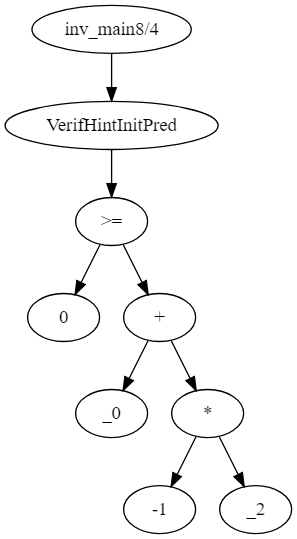
\includegraphics[width=3.4cm]{graph/template_graph}\\
  \subcaption{Template graph example}\label{templateGraph}
  \end{subfigure}
  \caption{Graph representation for an example template "inv\_main8:VerifHintInitPred(((\_0 + -1 * \_2) >= 0))"}
\end{figure}




\section{Data Collection}
For a single instance of data extracting from manual\cite{10.1007/978-3-319-57288-8_18} or simple heuristics\cite{Leroux2016}, the inputs are a list of templates $T_{0},T_{1},...,T_{n}$ and a program $P$. The output is a list of templates with 0 or 1 labels $T_{0}^{l},T_{1}^{l},...,T_{n}^{l}, l= 0$ or $1$. A concrete example for an output is $T_{0}^{1} = ("inv\_main8:VerifHintInitPred(((\_0 + -1 * \_2) >= 0))",1)$

\begin{algorithm}[H]
\SetAlgoLined
\KwResult{$T_{0}^{l},T_{1}^{l},...,T_{n}^{l}$}
 initialization:  CurrentTemplateList = $\{T_{0},T_{1},...,T_{n}\}$\;
 Solvalbility=CEGAR(CurrentTemplateList,HornClauses)\;
   \eIf{Solvalbility == True}{
    \While{CurrentTemplateList is not empty}{
        CurrentTemplateList = CurrentTemplateList $ - \{T_{k}\} (0\leqslant k \leqslant n)$\;
        Solvalbility=CEGAR(CurrentTemplateList,HornClauses)\;
        \eIf{Solvalbility == True}{
            RedunantTemplateList=RedunantTemplateList $\cup$ $T_{k}^{0}$;\
        }{
            CriticalTemplateList=CriticalTemplateList $\cup$ $T_{k}^{1}$;\
        }
        Templates=RedunantTemplateList $\cup$  CriticalTemplateList;\
    }
   }{
   Cannot solve within timeout, no template extracted\;
  }
 \caption{Templates extracting process}
\end{algorithm}

\begin{algorithm}[H]
\SetAlgoLined
\KwResult{$T_{0}^{l},T_{1}^{l},...,T_{n}^{l}$}
 initialization:  CurrentTemplateList = $\{T_{0},T_{1},...,T_{n}\}$\;
 Solvalbility,CurrentPredicateList=CEGAR(CurrentTemplateList,HornClauses)\;
   \eIf{Solvalbility == True}{
    \While{CurrentPredicateList is not empty}{
        CurrentPredicateList = CurrentPredicateList $ - \{P_{k}\} (0\leqslant k \leqslant n)$\;
        CurrentTemplateList=transform(CurrentPredicateList)
        Solvalbility=CEGAR(CurrentTemplateList,HornClauses)\;
        \eIf{Solvalbility == True}{
            RedunantPredicateList=RedunantPredicateList $\cup$ $P_{k}^{0}$;\
        }{
            CriticalPredicateList=CriticalPredicateList $\cup$ $P_{k}^{1}$;\
        }
    }
    Templates=transform(RedunantPredicateList $\cup$  CriticalPredicateList);\
   }{
   Cannot solve within timeout, no template extracted\;
  }
 \caption{Predicates extracting process}
\end{algorithm}

The final goal is to have proper predicates that can represent the abstract transition system. The templates are heuristics to generate the predicates in each CEGAR iteration. There are additional predicates added to solve the program in every CEGAR iterationl but the templates are given and fixed before the CEGAR iteration.

The strategy $A$ (fixed time out) to extract the training data (a list of templates with labels) is that for one program, we run Eldarica with an abstraction heuristic (e.g. use option -abstract:manual for .c files and -abstract for .smt2 files). If Eldarica can solve the program within 60 seconds. We mark this program as solvable. In Eldarica, we have an initial list of templates. We delete these templates one by one to see if the program can be solved with the remaining templates. If the program is still solvable within the timeout, then that deleted template is critical, we mark it as useful and label it as 1. By doing so iteratively, we can label the initial list of templates. This labelled list of templates will be used in the training process.

\begin{enumerate}
  \item chc-comp benchmarks: 38/1216 .smt2 files (programs) need templates to solve the program within in 60 seconds.
  \item sv-comp smt benchmarks: 7/6814 .smt2 files need templates.
  \item sv-comp c benchmarks: 31/545 .c files need templates.
\end{enumerate}

Only 76 training programs in total.

A alternative strategy $B$ (variable timeout): First, confirm the solvability (i.e. the program can be solved within 60 seconds with the abstraction heuristic).
Second, record the solving time with and without the abstraction heuristic. If Eldarica takes less solving time with abstraction heuristic, pass this solving time as timeout to Eldarica to label the templates used in the program.

\begin{enumerate}
  \item chc-comp benchmarks: 40/1216.  32 programs (204 templates)for training and 8 (47 templates) for testing. 8/8 solved by read templates. Read templates time consumption/original templates consumption =  40.25/40.86 (in seconds)
  \item sv-comp smt benchmarks: 15/5911.  12 programs (254 templates)for training and 3 (74 templates) for testing. 3/3 solved by read templates. Read templates time consumption/original templates consumption =  28.07/27.28 (in seconds)
  \item sv-comp c benchmarks: 41/555.  32 programs (4635 templates)for training and 9 (350 templates) for testing. 8/9 solved by read templates. Read templates time consumption/original templates consumption = 34.04/53.46  (in seconds)
\end{enumerate}

96 training programs. 76 programs for training, 20 programs for testing.
18/20 solved by read templates. Read templates time consumption/original templates consumption =  140.67/126.84 (in seconds)

Strategy $C$: keep using Strategy $B$'s on larger benchmarks, and use these three benchmarks only for testing.






We try to use balanced and imbalanced data set to train the neural network.

%\begin{table}
%\begin{center}\caption{Balanced Predicates}
%\begin{tabular}{lp{1.5cm}p{2cm}p{2cm}p{1.5cm}p{1.5cm}p{1.5cm}p{1.5cm}p{1.5cm}}
%\hline
%Benchmarks  & Training program &Testing program&Training  predicates & Testing predicates & Solved programs & Time consumption(predicated/abstract)\\
%\hline
%chc-comp-smt  &133/167&34/167&700/1174&474/1174& 34/34 & 105.4/105.2\\
%sv-comp-smt  &-&-&-&-\\
%sv-comp-c  &148 & 30 & 1482 & 1128& 23/30 & 3608&7796\\
%In total &-&-&-&-\\
%\hline
%\end{tabular}
%\end{center}
%\end{table}



\section{Training Model}


\begin{figure}[h]
\centering
  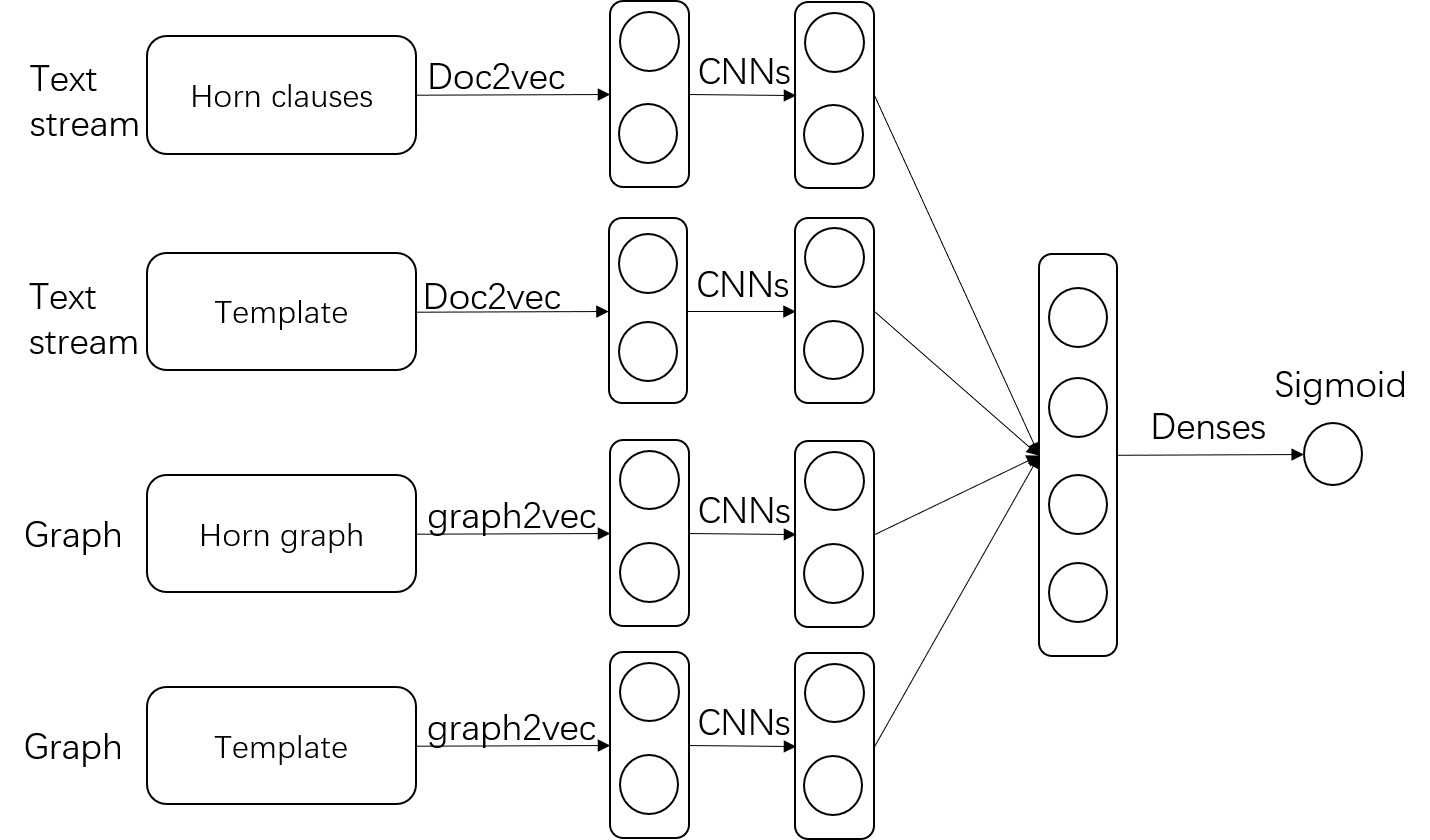
\includegraphics[width=10cm]{graph/NNstructure}\\
  \caption{Neural network structure}\label{NNstructure}
\end{figure}
\subsection{Program Embedding}

\subsubsection{Text Level}
Doc2Vec \cite{DBLP:journals/corr/LeM14} embed different length of sentences to fixed vector.
Program text streams are embedded into 100 dimensions. Template text streams are embedded to 20 dimensions.
\subsubsection{Graph Level}
Graph2Vec\cite{DBLP:journals/corr/NarayananCVCLJ17}.
WL relabeling process \cite{WL_relabeling_process} to generate random subgraphs (can be seen as sentences). Then use Doc2Vec embed subgraphs to fixed vector.
Program graphs (horn graphs) are embedded into 100 dimensions. Templates are embedded to 20 dimensions.



\section{Experiments}
The predicted result is a score for a template. We add two rank modes to decide which templates will be used for solving a particular program. For example, we have 10 templates, their scores ranged from 0 to 1. The first rank mode can specify a threshold for the scores. If the threshold is 0.4, all templates that have scores larger than 0.4 will be used to solve the program, and the left templates are discarded. The second rank mode can specify a hierarchical number (N) which decides to use top N ranked templates by score. If we specify the hierarchical number (N) be 5, then the top 5 ranked templates by score will be used to solve the program, and the left 5 templates will be discarded.

\subsection{Ablation studies}



\begin{table}\caption{Benchmarks}
\begin{center}
\begin{tabular}{lp{1cm}p{1cm}p{1.5cm}p{1.5cm}p{1.5cm}p{1.5cm}p{1.5cm}p{1.5cm}}
\hline
Benchmarks & File type & Total file & Solved & sat & unsat & Unsolved  \\
\hline
chc-comp-smt & .smt2 & 1216 & 421  & 339  & 82    & 795 \\
sv-comp-smt &.smt2   & 5911 & 4730 & 4516 & 214  & 1181 \\
sv-comp-c &.c        & 555  & 323  & 262  & 61   & 231 \\
In total  & - & - & -&-&-&-&-&-\\
\hline
\end{tabular}
\end{center}
\end{table}


\begin{table}[h]
\begin{center}\caption{Imbalanced Predicates with control flow and template graph}
\begin{tabular}{lp{1.5cm}p{2cm}p{2cm}p{1.5cm}p{1.5cm}p{2.5cm}}
\hline
Benchmarks  & Training program &Testing program&Training  predicates & Testing predicates & Solved programs & Total time consumption (predicted:abstract)\\
\hline
chc-comp-smt  & 130 & 33& 969 & 225 & 33/33 & 63.92 : 63.72 (s)\\
sv-comp-smt  &784 &196 & 5907 & 1406 & 196/196 & 514.60 : 511.186 \\
sv-comp-c  &116 & 29  & 4148 & 847 & 20/29 &  578.33 : 56.74  \\
In total  & 1030 & 258 & 10588 & 2914 & 250/258 & 1119.73 : 629.82 \\
\hline
\end{tabular}
\end{center}
\end{table}


\begin{table}[h]
\begin{center}\caption{Imbalanced Templates with control flow and template graph}
\begin{tabular}{lp{1.5cm}p{2cm}p{2cm}p{1.5cm}p{1.5cm}p{2.5cm}}
\hline
Benchmarks  & Training program &Testing program&Training  predicates & Testing predicates & Solved programs & Time consumption (predicted/abstract)\\
\hline
chc-comp-smt  &- &- &- & - & - & - (s)\\
sv-comp-smt  &-&-&-&-&-&-\\
sv-comp-c  &- &- & - &-&-&-\\
In total &-&-&-&-\\
\hline
\end{tabular}
\end{center}
\end{table}






CEGAR iterations:

Solvability:
\begin{center}
\begin{tabular}{lp{1cm}p{1cm}p{1cm}p{1cm}p{1cm}p{1cm}p{1cm} }
\hline
Benchmarks  & Total file & with template graph & with horn graph & with control flow graph &with control flow and template graphs & with horn and template graphs\\
\hline
chc-comp-smt & 1216 & -&-\\
sv-comp-smt & 5911 & -&-\\
sv-comp-c  & 555 & -&-\\
\hline
\end{tabular}
\end{center}

Time consumption:
\begin{center}
\begin{tabular}{lp{1cm}p{1cm}p{1cm}p{1cm}p{1cm}p{1cm}p{1cm} }
\hline
Benchmarks  & Total file & with template graph & with horn graph & with control flow graph &with control flow and template graphs & with horn and template graphs\\
\hline
chc-comp-smt  & 1216 & -&-\\
sv-comp-smt  & 5911 & -&-\\
sv-comp-c  & 555 & -&-\\
\hline
\end{tabular}
\end{center}

\section{Related work}

Text level learning for improving ATP (formal verification?) \cite{NIPS2016_6280}

Guiding formal method's search process.

Program graph representation.

end-to-end graph embedding. Message passing, convolutional graph neural network.
Define a the first state of nodes. Update node representations by edges type and the connected node. Iteration is intuitively the filters of CNNs.
The edges, hyper-edges, messages should capture the characteristics or relations between nodes.
To deal with arbitrary length of information (different number of nodes), aggregation or abstraction then aggregation.

AST embedding: code2vec \cite{Alon:2019:CLD:3302515.3290353}. TBCNN \cite{DBLP:journals/corr/MouLJZW14}.


FormulaNet \cite{NIPS2017_6871}. GAT \cite{2017arXiv171010903V}.
Gated Graph Neural Networks (GGNN) \cite{DBLP:journals/corr/abs-1711-00740}

fake task graph embedding.




%Program synthesis:
%
%Logical reasoning: NEO, BLAZE, CEGIS.
%
%Machine learning methods:
%Program synthesis from examples:
%Encode inputs to fixed vector, then decode this vector to target language.
%
%Program induction:
%Directly give output. The learned program is induced latently within the weights and activations of a neural network.
%
%Guide formal method's search process by Training a statistical model to rank some options existed in search space and try them first.


\section{Discussion and Future work}
%
%
%\section{Headings: first level}
%\label{sec:headings}
%
%\lipsum[4] See Section \ref{sec:headings}.
%
%\subsection{Headings: second level}
%\lipsum[5]
%\begin{equation}
%\xi _{ij}(t)=P(x_{t}=i,x_{t+1}=j|y,v,w;\theta)= {\frac {\alpha _{i}(t)a^{w_t}_{ij}\beta _{j}(t+1)b^{v_{t+1}}_{j}(y_{t+1})}{\sum _{i=1}^{N} \sum _{j=1}^{N} \alpha _{i}(t)a^{w_t}_{ij}\beta _{j}(t+1)b^{v_{t+1}}_{j}(y_{t+1})}}
%\end{equation}
%
%\subsubsection{Headings: third level}
%\lipsum[6]
%
%\paragraph{Paragraph}
%\lipsum[7]
%
%\section{Examples of citations, figures, tables, references}
%\label{sec:others}
%\lipsum[8] \cite{kour2014real,kour2014fast} and see \cite{hadash2018estimate}.
%
%The documentation for \verb+natbib+ may be found at
%\begin{center}
%  \url{http://mirrors.ctan.org/macros/latex/contrib/natbib/natnotes.pdf}
%\end{center}
%Of note is the command \verb+\citet+, which produces citations
%appropriate for use in inline text.  For example,
%\begin{verbatim}
%   \citet{hasselmo} investigated\dots
%\end{verbatim}
%produces
%\begin{quote}
%  Hasselmo, et al.\ (1995) investigated\dots
%\end{quote}
%
%\begin{center}
%  \url{https://www.ctan.org/pkg/booktabs}
%\end{center}
%
%
%\subsection{Figures}
%\lipsum[10]
%See Figure \ref{fig:fig1}. Here is how you add footnotes. \footnote{Sample of the first footnote.}
%\lipsum[11]
%
%\begin{figure}
%  \centering
%  \fbox{\rule[-.5cm]{4cm}{4cm} \rule[-.5cm]{4cm}{0cm}}
%  \caption{Sample figure caption.}
%  \label{fig:fig1}
%\end{figure}
%
%\subsection{Tables}
%\lipsum[12]
%See awesome Table~\ref{tab:table}.
%
%\begin{table}
% \caption{Sample table title}
%  \centering
%  \begin{tabular}{lll}
%    \toprule
%    \multicolumn{2}{c}{Part}                   \\
%    \cmidrule(r){1-2}
%    Name     & Description     & Size ($\mu$m) \\
%    \midrule
%    Dendrite & Input terminal  & $\sim$100     \\
%    Axon     & Output terminal & $\sim$10      \\
%    Soma     & Cell body       & up to $10^6$  \\
%    \bottomrule
%  \end{tabular}
%  \label{tab:table}
%\end{table}
%
%\subsection{Lists}
%\begin{itemize}
%\item Lorem ipsum dolor sit amet
%\item consectetur adipiscing elit.
%\item Aliquam dignissim blandit est, in dictum tortor gravida eget. In ac rutrum magna.
%\end{itemize}


\bibliographystyle{unsrt}
%\bibliography{references}  %%% Remove comment to use the external .bib file (using bibtex).
%%% and comment out the ``thebibliography'' section.

\bibliography{references}
%%% Comment out this section when you \bibliography{references} is enabled.
%\begin{thebibliography}{1}
%
%\bibitem{kour2014real}
%George Kour and Raid Saabne.
%\newblock Real-time segmentation of on-line handwritten arabic script.
%\newblock In {\em Frontiers in Handwriting Recognition (ICFHR), 2014 14th
%  International Conference on}, pages 417--422. IEEE, 2014.
%
%\bibitem{kour2014fast}
%George Kour and Raid Saabne.
%\newblock Fast classification of handwritten on-line arabic characters.
%\newblock In {\em Soft Computing and Pattern Recognition (SoCPaR), 2014 6th
%  International Conference of}, pages 312--318. IEEE, 2014.
%
%\bibitem{hadash2018estimate}
%Guy Hadash, Einat Kermany, Boaz Carmeli, Ofer Lavi, George Kour, and Alon
%  Jacovi.
%\newblock Estimate and replace: A novel approach to integrating deep neural
%  networks with existing applications.
%\newblock {\em arXiv preprint arXiv:1804.09028}, 2018.
%
%\end{thebibliography}


\end{document}
